
\chapter{star\_tp}
\label{chap:startp3}

在多核的共享内存环境下,并行优化要达到较高的优化结果,就要减少同步造成的CPU时间浪费,充分挖掘计算资源的利用率。star\_tp是共享内存下基于数据流计算模型的并行优化系统,采用线程池技术实现,它的运行时系统提供高效的任务调度策略,没有依赖的任务可以在计算资源充足的情况下异步执行,充分利用计算资源。下面从架构的设计、API风格和功能性测试等方面介绍star\_tp。

\section{star\_tp的架构}

star\_tp的架构如图3.1所示。

\begin{figure}[!htbp]
    \centering
    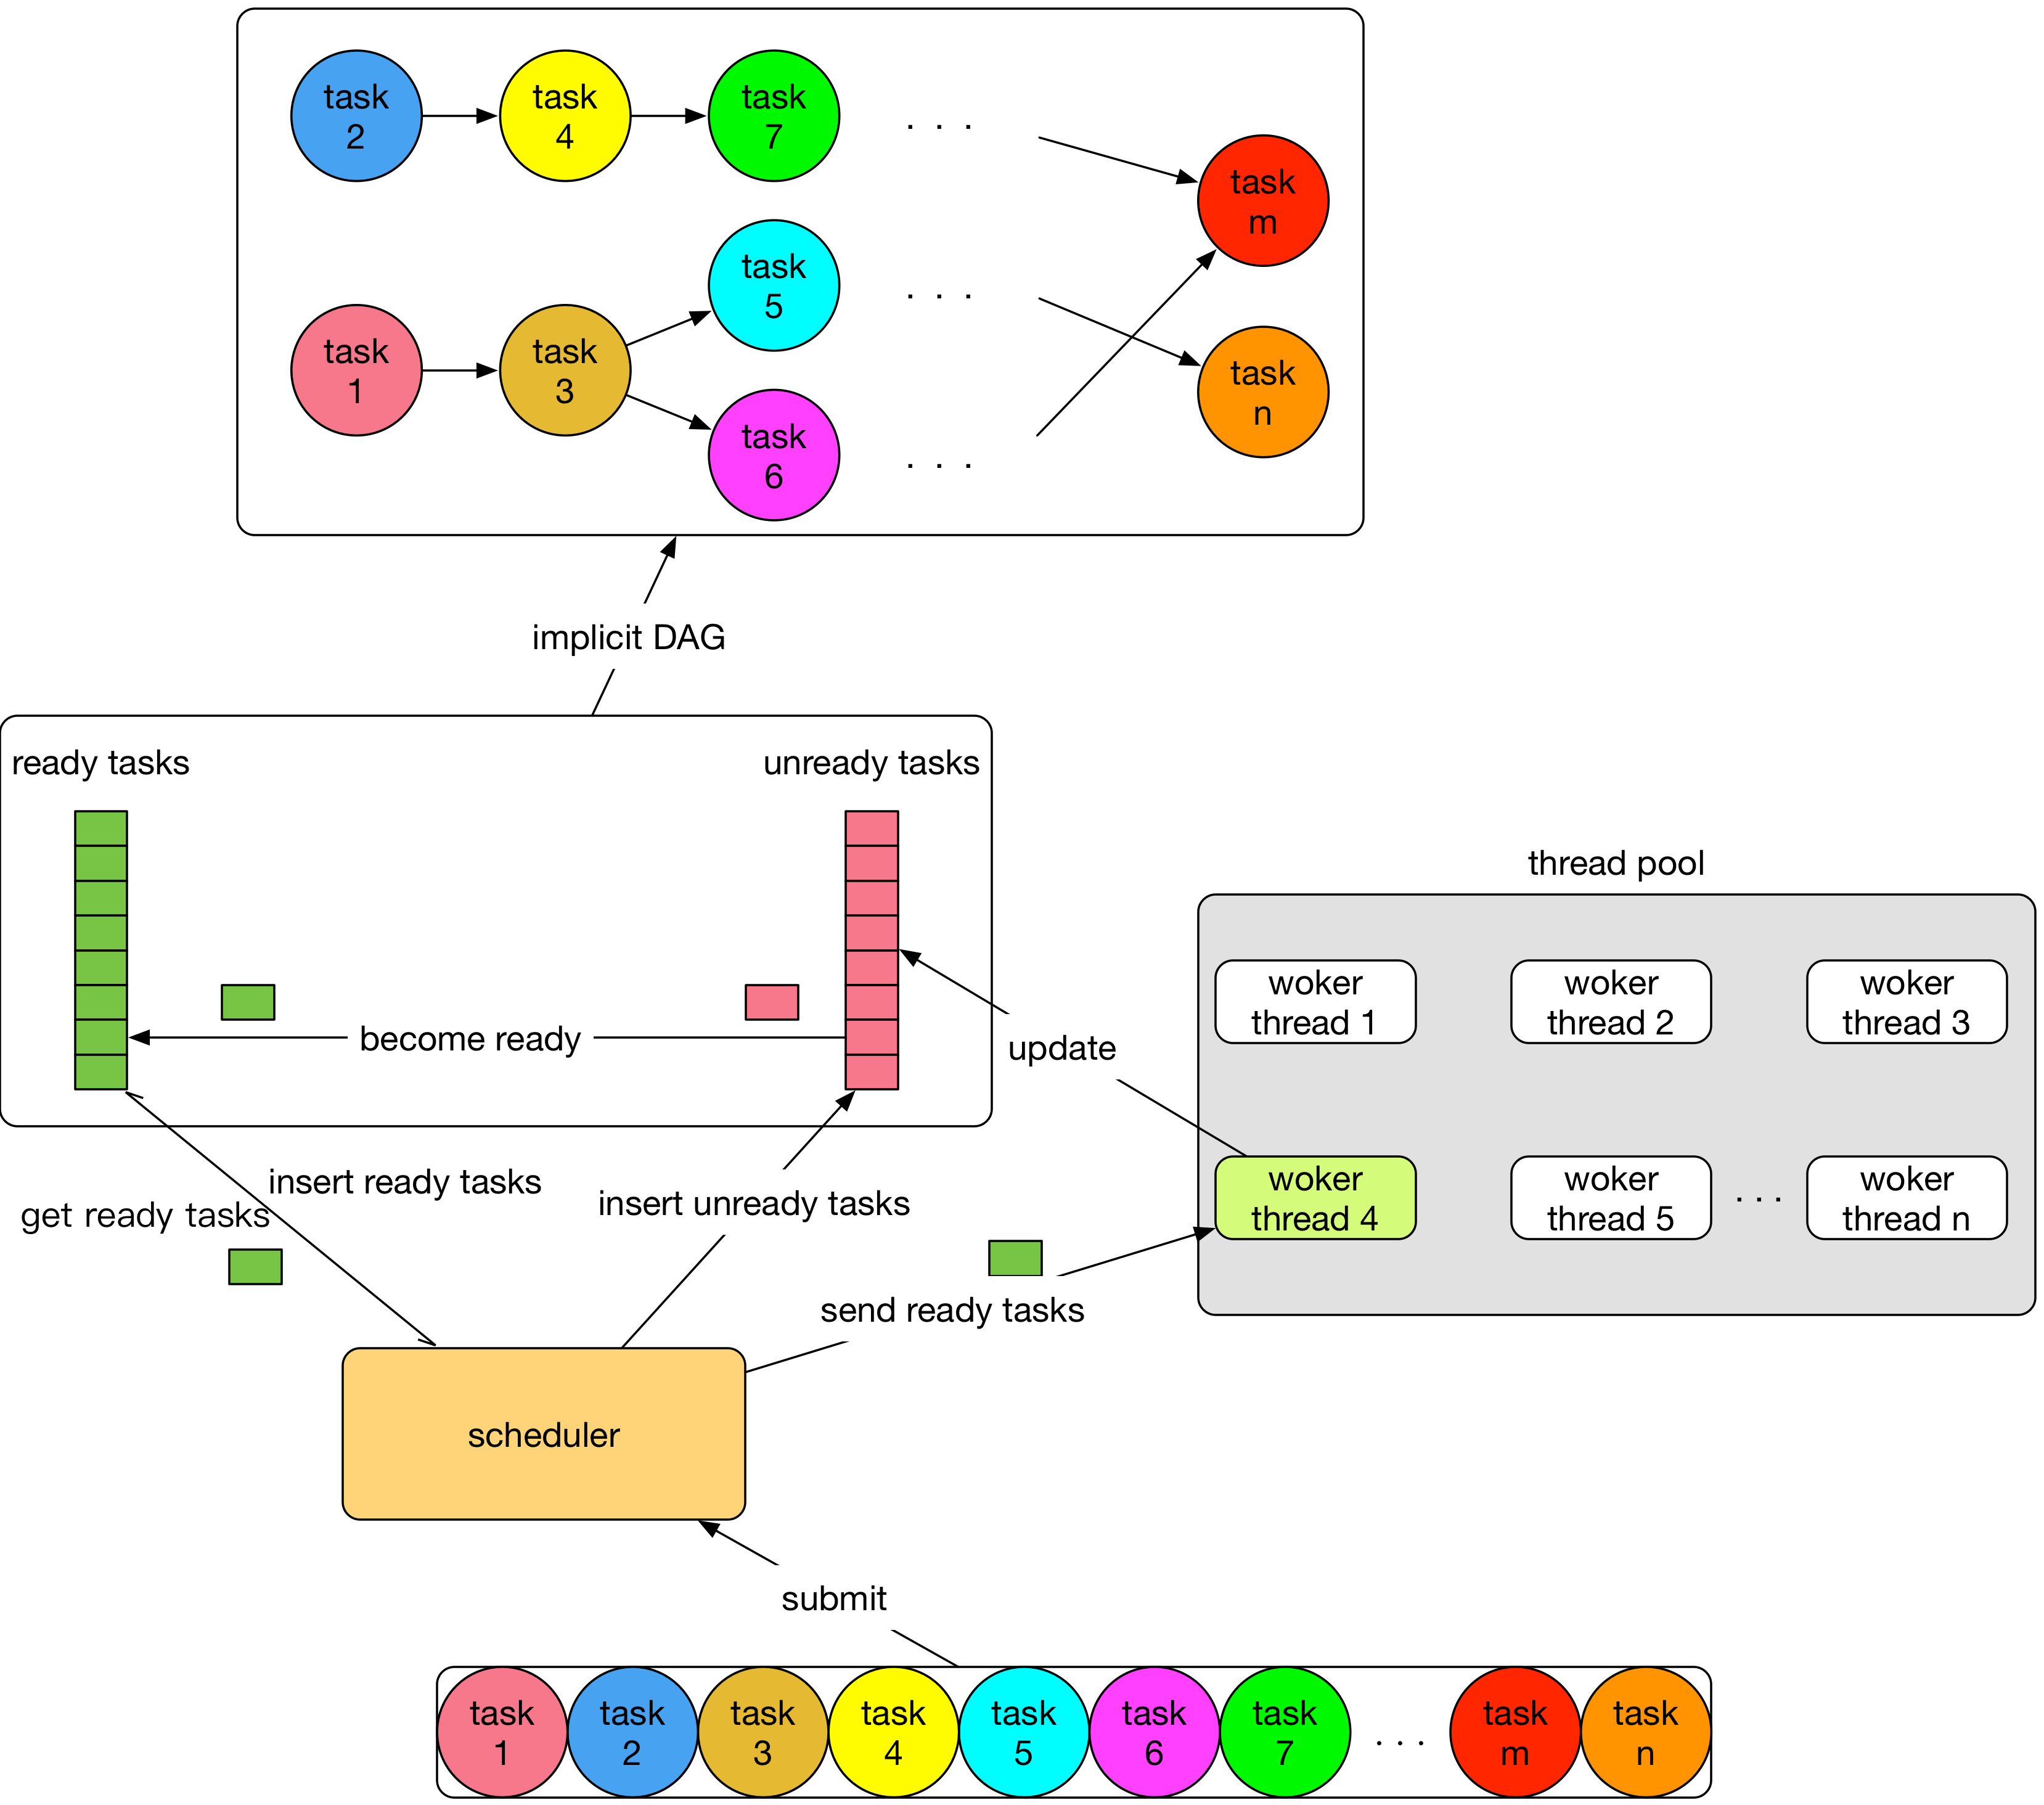
\includegraphics[width=0.60\textwidth]{3_star_tp-architecture}
    \bicaption{star\_tp的架构。}{Architecture of star\_tp.}
    \label{fig:3_star_tp-architecture}
\end{figure}

star\_tp的架构主要由四个模块组成:

\begin{enumerate}
	\item 线程池:在star\_tp运行时环境初始化时创建一组线程,程序运行时负责线程的分发和回收,退出运行时环境时销毁线程资源。
	\item 任务队列:线程安全的数据结构,分为就绪任务队列和未就绪任务队列。
	\item 调度器:插入任务,获取更新后的DAG,将就绪任务分发给worker线程,等待所有任务执行完成。
	\item worker线程:执行调度器发送来的任务,更新DAG。
\end{enumerate}

\subsection{线程池}

创建进程的系统开销要比创建线程大的多,一般有成百上千倍的差距\citep{Ling:2000:AOT:346152.346320},所以共享内存环境下的并行优化一般采用多线程。在实现star\_tp的时候我采用线程池来实现多线程并行优化,采用线程池而不是直接操作每个线程的原因如下:

\begin{itemize}
	\item 创建和销毁线程伴随着系统开销,过于频繁的创建或销毁线程,会很大程度上影响处理效率,线程池的使用可以减少这些开销;
	\item 每个活动的线程都会占用一定的系统资源,如果线程并发数量过多,会抢占过多系统资源从而导致阻塞;
	\item 通过对有限个线程的重用,线程创建和销毁的开销就可以分摊到多个任务上,使worker线程的响应更快;
	\item 能够对线程进行简单的管理并提供定时执行、间隔执行等功能。
\end{itemize}

如图3.1所示,star\_tp中的线程池是一组固定数量的线程,每个线程上都有一个worker在运行着。线程池提供提交任务的接口,当有任务到来时,线程池会将任务分配到一个空闲的worker上执行,如果所有的worker都处于工作状态,线程池就会阻塞,直到有空闲的worker接收这个任务。

由于线程池是单例,所以不用考虑线程池分配任务时的线程安全问题。这样设计的原因是,在实际应用场景中,共享内存环境下的物理核数一般都是几十到几百个,线程池的容量一般也设置为小于实际物理核数,避免过多的线程造成系统资源抢占,导致性能下降。所以单例模式足以用来管理正常容量的线程池。

\subsection{任务队列}

任务封装了要执行的函数和参数,每个任务对象都包含流入自己和流出自己的依赖关系,所有任务之间的依赖关系构成了一个隐式的DAG(有向无环图)。由于对任务队列的访问是并发的,所以要保证任务队列的线程安全。一旦任务队列是线程安全的,调度器更新任务依赖的逻辑就变得简单多了。

任务队列的底层数据结构是线程安全的队列,通过互斥锁来实现。对于push操作,首先获得队列的互斥锁,然后将元素入队,最后释放锁。对于pop操作,提供了非阻塞pop和阻塞pop两种方式:非阻塞pop首先获得队列的互斥锁,然后检查队列是否为空,若为空则返回空,否则返回队首元素并将队首元素出队;阻塞pop则一直等到队列不为空才锁住队列并执行pop操作。

\subsection{调度器}

调度器是负责任务调度的模块,主要功能包括:

\begin{enumerate}
	\item 插入任务:开始进行任务调度之前,需要先定义所有任务,根据任务的原始状态初始化就绪任务队列和未就绪任务队列。调度器的插入任务的接口的作用就是初始化任务队列。
	\item 发送任务:从就绪任务队列中获取任务,并将就绪任务发送到线程池。
	\item 更新DAG:如果就绪任务队列为空,未就绪队列不为空,说明需要更新DAG,已完成的任务造成的依赖关系的改变会导致未就绪任务转为就绪任务。
	\item 等待退出:当任务队列(包括就绪任务队列和未就绪任务队列)为空时,说明任务调度阶段结束,等待所有worker线程执行完各自的当前任务后退出就可以了。
\end{enumerate}

\subsection{worker线程}

worker线程负责任务的执行和相关依赖关系的更新,worker的整个生命周期都处于下面三种状态:

\begin{enumerate}
	\item 休眠状态:当没有获得任务时,worker处于休眠状态;
	\item 执行状态:获得任务后,worker首先从任务中获取要执行的任务的具体内容,包括要执行的函数和参数,然后执行对应的函数;
	\item 更新状态:执行完任务后还要更新跟这个任务相关的依赖。举例说明:设当前任务是a,另一个任务b依赖a,那么当a执行完成后,就可以从b的依赖集中移除a,如果此时b的依赖集为空,意味着b由未就绪状态转为就绪状态,需要将b移入就绪任务队列,等待调度器进行调度。
\end{enumerate}

\section{高效的DAG更新策略}

star\_tp中的任务的状态有两种:就绪和未就绪。运行时任务之间的依赖关系会构成一个隐式的DAG,任务调度的过程中,需要不断的更新DAG,及时将依赖已经满足的未就绪任务的状态转换为就绪。如果更新过慢,worker就不能及时接收到待执行任务,导致整体性能下降。所以要尽量优化DAG的更新策略,加速任务之间依赖关系的更新,使更多的worker同时保持执行任务状态。

star\_tp的架构是典型的master/slave架构,调度器是master,worker线程是slave。调度器负责更新DAG,随着任务数量的增加,DAG的规模会急剧增大,调度器的负载就会增加,成为性能瓶颈,这将降低master和slave之前的响应速度。为了减轻调度器的负担,单个任务状态的更新交给worker,worker执行完一个task之后,就会更新这个task流入和流出的依赖集,从而更新任务的状态(就绪或未就绪)。这样做的话,当调度器更新DAG时,只需要获取任务的状态就可以,而不用更新任务持有的依赖集。

采用这种DAG更新策略后,虽然调度器的负担就减轻了许多,但是更多的负担落到了任务队列上。因为将DAG更新的部分工作分担到worker上后,任务队列的并发访问频率就成倍增加了。但是在worker数量不多(100以下)的情况下,这种并发度完全不会造成性能瓶颈。

\section{star\_tp的API}

下面介绍star\_tp为用户提供的API。

\subsection{任务--CTask}

CTask是star\_tp中任务的封装,它提供的接口如图3.2所示。

\begin{figure}[!htbp]
    \centering
\begin{lstlisting}[language=c++,caption={}]
class CTask {
private:
    std::function<void()> mFunc;
    std::unordered_set<CTask*> mInDep, mOutDep;
    bool mDone;
    std::mutex mutInDep, mutOutDep, mutDone;
    CTask& addInDep(CTask*);
    void removeInDep(CTask*);
public:
    explicit CTask(std::function<void()>);
    ~CTask();
    bool isReady();
    bool isDone();
    CTask& addOutDep(CTask*);
    void operator()();
    void taskInfo();
};
\end{lstlisting}
    \bicaption{CTask。}{ CTask.}
    \label{fig:3_ctask}
\end{figure}

主要API解释:

\begin{itemize}
	\item 显示的构造函数:传入返回值为void的函数。
	\item isReady():任务是否就绪。
	\item isDone():任务是否已完成。
	\item addOutDep():添加依赖。
	\item operator()():执行任务。
\end{itemize}

\subsection{线程池--CThreadPool}

CThreadPool是star\_tp中的线程池类,它提供的接口如图3.3所示。

\begin{figure}[!htbp]
    \centering
\begin{lstlisting}[language=c++,caption={}]
class CThreadPool {
private:
    boost::thread_group mWorkers;
    boost::asio::io_service mIoService;
    boost::shared_ptr<boost::asio::io_service::work> mWork;
public:
    explicit CThreadPool(size_t);
    ~CThreadPool();
    void submit(CTask*);
    void submit(boost::function<void()>);
};
\end{lstlisting}
    \bicaption{CThreadpool。}{ CThreadpool.}
    \label{fig:3_cthreadpool}
\end{figure}

主要API解释:

\begin{itemize}
	\item 显示的构造函数:传入线程池容量,创建线程池。
	\item submit():向线程池提交任务(此时的任务认为已经ready,submit一般由scheduler代理)。
\end{itemize}

\subsection{调度器--CScheduler}

CScheduler是star\_tp中的调度器类,它提供的接口如图3.4所示。

\begin{figure}[!htbp]
    \centering
\begin{lstlisting}[language=c++,caption={}]
class CScheduler {
  private:
    CScheduler() {}
    CScheduler(const CScheduler &) {}
    CScheduler &operator=(const CScheduler &) {}
    ~CScheduler() {}
    static CThreadSafeQueue<CTask *> notReadyTaskQueue;
    static CThreadSafeQueue<CTask *> readyTaskQueue;
    static CScheduler *m_instance;
    static std::once_flag onceFlag;
    static void init();
    void updateNotReadyTasks();
    std::shared_ptr<CTask*> getReadyTask();
  public:
    static CScheduler *getInstance();
    void addTask(CTask*);
    void schedule(CThreadPool&);
};
\end{lstlisting}
    \bicaption{CScheduler。}{ CScheduler.}
    \label{fig:3_cscheduler}
\end{figure}

主要API解释:

\begin{itemize}
	\item getInstance():获取CScheduler对象(CScheduler是单例)。
	\item addTask():添加任务(初始化任务队列)。
	\item schedule():向scheduler注册对应的线程池,开始进行任务调度,直到所有任务执行完成。
\end{itemize}

\section{star\_tp的正确性测试}

对star\_tp进行正确性测试的主要目的就是验证star\_tp中的任务调度机制是否运行正确,即任务执行的顺序是否符合运行时DAG的状态。下面以图3.5所示的测试用例为例进行正确性测试。在图3.5中,每个节点代表一个任务,一共有16个任务,节点上的数字代表task id;箭头表示相连的两个任务之间存在依赖关系;每个任务的内容是休眠1秒,然后打印task id。

如何来判断程序的运行结果是否正确呢?以图3.5为例,像task 0,task 2,task 6这样的任务,他们的输入依赖为空,在程序运行时只要有空闲的worker就可以立即并行执行;但是像task 3 这样的任务,它的输入依赖是task 1和task 2,只有当task 1和task 2完成后task 3才可以开始执行。所以只要不违背上述的任务执行顺序,就说明star\_tp任务调度算法是正确的。

\begin{figure}[!htbp]
    \centering
    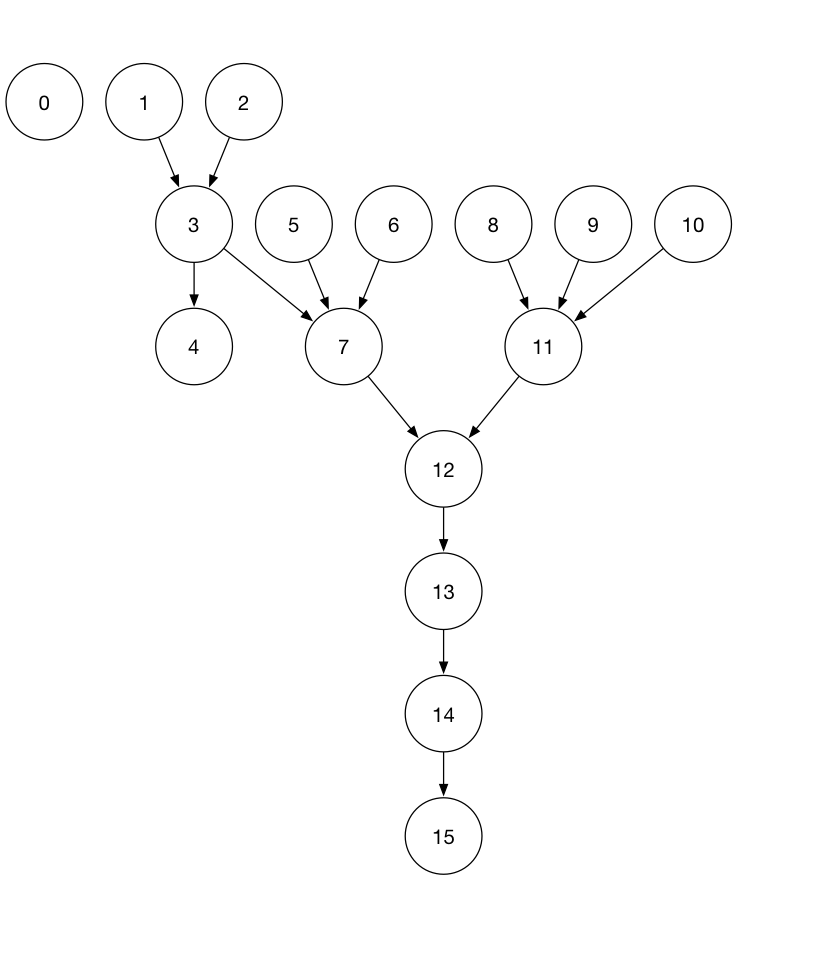
\includegraphics[width=0.60\textwidth]{3_star_tp_example_topo}
    \bicaption{star\_tp测试用例任务拓扑。}{ Task topology of star\_tp test case.}
    \label{fig:3_star_tp_example_topo}
\end{figure}

图3.5的测试用例任务拓扑图对应的测试代码如图3.6所示,这是使用star\_tp进行并行优化的典型代码结构。下面逐行解释图3.6中的测试代码:

\begin{itemize}
	\item \textbf{第1-4行}:待执行函数的定义。
	\item \textbf{第6行}:构造线程池,指定线程池容量为6,将创建6个worker线程。
	\item \textbf{第7行}:获取调度器单例对象。
	\item \textbf{第8-10行}:定义所有任务。
	\item \textbf{第11-23行}:指定任务之间的依赖关系。
	\item \textbf{第24行}:调度器插入任务。
	\item \textbf{第25行}:调度器绑定线程池,开始进行任务调度,直到所有任务完成。
\end{itemize}

\begin{figure}[!htbp]
    \centering
\begin{lstlisting}[language=c++,caption={}]
static void taskDemo(int taskId) {
    sleep(1);
    printf("task %d\n", taskId);
}
int main() {
    CThreadPool pool(6);
    CScheduler * schdp = CScheduler::getInstance();
    char * p = new char[sizeof(CTask)*16];
    CTask* taskVector = (CTask*)p;
    for (int i = 0; i < 16; ++i) new (taskVector+i)CTask(std::function<void()>(std::bind(taskDemo, i)));
    taskVector[1].addOutDep(&taskVector[3]);
    taskVector[2].addOutDep(&taskVector[3]);
    taskVector[3].addOutDep(&taskVector[4]).addOutDep(&taskVector[7]);
    taskVector[5].addOutDep(&taskVector[7]);
    taskVector[6].addOutDep(&taskVector[7]);
    taskVector[8].addOutDep(&taskVector[11]);
    taskVector[9].addOutDep(&taskVector[11]);
    taskVector[10].addOutDep(&taskVector[11]);
    taskVector[7].addOutDep(&taskVector[12]);
    taskVector[11].addOutDep(&taskVector[12]);
    taskVector[12].addOutDep(&taskVector[13]);
    taskVector[13].addOutDep(&taskVector[14]);
    taskVector[14].addOutDep(&taskVector[15]);
    for (int i = 0; i < 16; ++i) schdp->addTask(&taskVector[i]);
    schdp->schedule(pool);
    delete [] p;
    return 0;
}
\end{lstlisting}
    \bicaption{star\_tp测试代码。}{ Test code of star\_tp.}
    \label{fig:3_star_tp_example_code}
\end{figure}

测试程序运行在有64个核的服务器上,由于线程池容量指定为6,所以不会出现线程资源抢占的情况。

运行结果如图3.7所示。在开始和退出阶段稍有停顿,这是因为star\_tp运行时环境的初始化和退出阶段涉及许多资源的申请和释放。

\begin{figure}[!htbp]
    \centering
    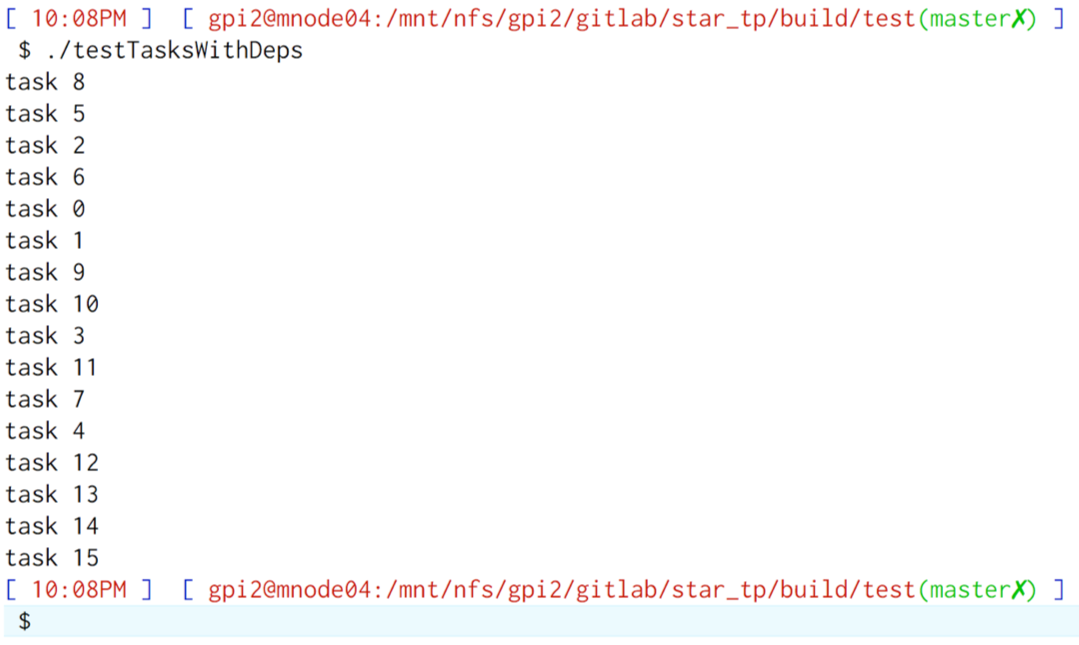
\includegraphics[width=0.60\textwidth]{3_star_tp_example_result}
    \bicaption{star\_tp测试用例运行结果。}{ Result of star\_tp test case.}
    \label{fig:3_star_tp_example_result}
\end{figure}

程序多次执行的结果是不同的,因为可以并行执行的任务的执行顺序是不固定的。但是线程池容量确定的情况下,这个测试用例的运行过程可以分为七个阶段,如表3.1所示。在线程池容量为6时,运行结果如视频和右图所示。

\begin{table}[!htbp]
    \bicaption{star\_tp测试用例的七个运行阶段。}{Seven running phases of star\_tp test case.}
    \label{tab:sample}
    \centering
    \footnotesize
    \setlength{\tabcolsep}{4pt}
    \renewcommand{\arraystretch}{1.2} 
    \begin{tabular}{lcccccccc}
        \hline
        运行阶段编号 & 运行的任务 \\
        %\cline{2-9}% partial hline from column i to column j
        \hline
        1 & 0,1,2,5,6,8\\
        2 & 3,9,10\\
        3 & 4,7,11\\
        4 & 12\\
        5 & 13\\
        6 & 14\\
        7 & 15\\
        \hline
    \end{tabular}
\end{table}

程序执行的七个阶段的运行时情景是这样的:程序开始运行后,0,1,2,5,6,8,9,10这些任务都是就绪的,但是由于线程池容量有限,前六个先执行,由于9,10两个任务在其他任务之后插入任务队列,所以调度的时候也排在后边;然后(约一秒后),已经就绪的9和10立即执行,由于1和2执行完成,变为ready的3也执行了……依次类推,任务的调度和执行按照指定的依赖关系异步并行执行。


